% LaTeX path to the root directory of the current project, from the directory in which this file resides
% and path to econtexPaths which defines the rest of the paths like \FigDir
\providecommand{\econtexRoot}{}\renewcommand{\econtexRoot}{.}

\documentclass[\econtexRoot/Letter]{subfiles}
\onlyinsubfile{\externaldocument{\econtexRoot/Letter}} % Get xrefs -- esp to apndx -- from main file; only works if main file has already been compiled

\begin{document}
\notinsubfile{\renewcommand{\econtexRoot}{.}}

%\hypertarget{model}{}\par\section{Model}
%\notinsubfile{\label{sec:model}}

[Description of JMP and any other relevant work] \\

William's job market paper evaluates the macroeconomic consequences of the long lasting negative effects of unemployment on labor earnings in the transmission unemployment risk as a business cycle amplifier and in the transmission of UI as a macroeconomic stabilizer. To do so, he builds a heterogeneous agent New Keynesian (HANK) model with search and matching frictions augmented to include human capital dynamics. His model matches the persistent earnings loss following job displacement that is present in the data, the path of IMPCs documented in Norwegian data, and the distribution of liquid wealth consistent with the Survey of Consumer Finances. With the model in hand, he shows that precautionary saving in response to heightened unemployment risk is substantially larger when households are subject to long term earnings loss following job displacement. Over the business cycle, he demonstrates that unemployment risk is a much stronger amplifier of fluctuations and that UI multipliers rise with the policy horizon largely due to their effect on expectations as opposed to their stimulative effect on income. For longer policy horizons, he finds that extending UI is considerably more stimulative than increasing the UI replacement rate as it precisely mitigates the precautionary saving that arises against the possibility of long term unemployment. 


%\textbf{ \large JMP Abstract}\\

%Unemployment has long lasting negative effects on labor earnings that persists even after reemployment. In this paper, I study the macroeconomic consequences of these microeconomic effects on business cycle fluctuations and in the transmission of unemployment insurance policies. Using a heterogeneous agent New Keynesian (HANK) model with search and matching frictions augmented to include human capital dynamics, I show that precautionary saving in response to heightened unemployment risk is substantially larger when households are subject to long term earnings loss following job displacement. Over the business cycle, unemployment risk is a much stronger amplifier of fluctuations and UI multipliers rise with the policy horizon largely due to their effect on expectations as opposed to their stimulative effect on income. For longer policy horizons, extending UI is considerably more stimulative than increasing the UI replacement rate as it precisely mitigates the precautionary saving that arises against the possibility of long term unemployment. 


%%% Figures below:
%\begin{figure}[ht!]
%	\centering
%	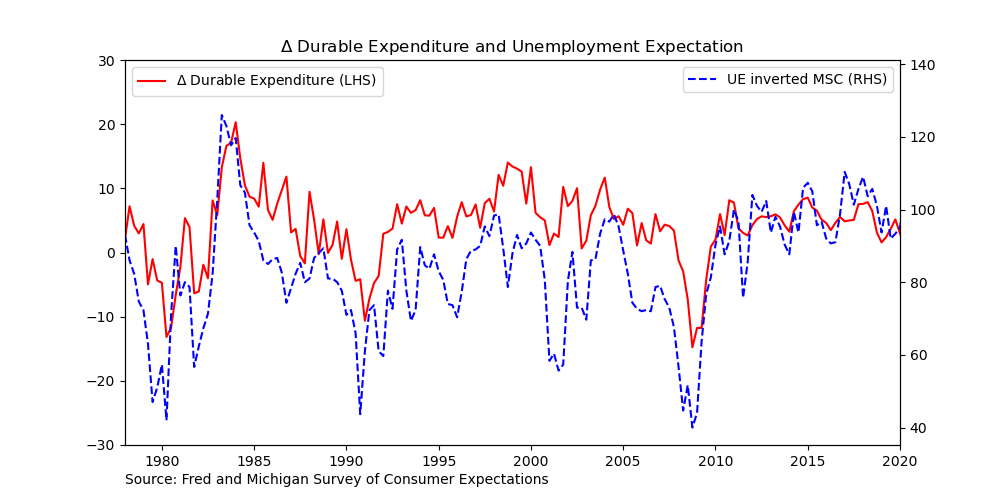
\includegraphics[width = 0.8\textwidth]{\FigDir/dur_vs_exp_emp.png}
	%\caption{Durable Expenditure and Expected Unemployment Rate} \label{fig:dur_vs_exp_emp}
%\end{figure}

\onlyinsubfile{% Allows two (optional) supplements to hard-wired \texname.bib bibfile:
% system.bib is a default bibfile that supplies anything missing elsewhere
% Add-Refs.bib is an override bibfile that supplants anything in \texfile.bib or system.bib
\provideboolean{AddRefsExists}
\provideboolean{systemExists}
\provideboolean{BothExist}
\provideboolean{NeitherExists}
\setboolean{BothExist}{true}
\setboolean{NeitherExists}{true}

\IfFileExists{\econtexRoot/Add-Refs.bib}{
  % then
  \typeout{References in Add-Refs.bib will take precedence over those elsewhere}
  \setboolean{AddRefsExists}{true}
  \setboolean{NeitherExists}{false} % Default is true
}{
  % else
  \setboolean{AddRefsExists}{false} % No added refs exist so defaults will be used
  \setboolean{BothExist}{false}     % Default is that Add-Refs and system.bib both exist
}

% Deal with case where system.bib is found by kpsewhich
\IfFileExists{/usr/local/texlive/texmf-local/bibtex/bib/system.bib}{
  % then
  \typeout{References in system.bib will be used for items not found elsewhere}
  \setboolean{systemExists}{true}
  \setboolean{NeitherExists}{false}
}{
  % else
  \typeout{Found no system database file}
  \setboolean{systemExists}{false}
  \setboolean{BothExist}{false}
}

\ifthenelse{\boolean{showPageHead}}{ %then
  \clearpairofpagestyles % No header for references pages
  }{} % No head has been set to clear

\ifthenelse{\boolean{BothExist}}{
  % then use both
  \typeout{bibliography{\econtexRoot/Add-Refs,\econtexRoot/\texname,system}}
  \bibliography{\econtexRoot/Add-Refs,\econtexRoot/\texname,system}
  % else both do not exist
}{ % maybe neither does?
  \ifthenelse{\boolean{NeitherExists}}{
    \typeout{bibliography{\texname}}
    \bibliography{\texname}}{
    % no -- at least one exists
    \ifthenelse{\boolean{AddRefsExists}}{
      \typeout{bibliography{\econtexRoot/Add-Refs,\econtexRoot/\texname}}
      \bibliography{\econtexRoot/Add-Refs,\econtexRoot/\texname}}{
      \typeout{bibliography{\econtexRoot/\texname,system}}
      \bibliography{        \econtexRoot/\texname,system}}
  } % end of picking the one that exists
} % end of testing whether neither exists
}

\ifthenelse{\boolean{Web}}{}{
  \onlyinsubfile{\captionsetup[figure]{list=no}}
  \onlyinsubfile{\captionsetup[table]{list=no}}
  \end{document}	\endinput
}

